\documentclass[11pt,a4paper]{article}

% ---------- Packages ----------
\usepackage[utf8]{inputenc}
\usepackage[T1]{fontenc}
\usepackage{lmodern}
\usepackage{amsmath,amssymb}
\usepackage{enumitem}
\usepackage{geometry}
\usepackage{fancyhdr}
\usepackage[most]{tcolorbox}   % enhanced, breakable
\usepackage{hyperref}
\usepackage[siunitx]{circuitikz}

% ---------- Geometry ----------
\geometry{margin=2.5cm}

% ---------- Header/Footer ----------
\setlength{\headheight}{14pt}  % fancyhdr warning verhindern
\pagestyle{fancy}
\fancyhf{}
\lhead{Introduction to Electrical Engineering}
\cfoot{\thepage}

% ---------- Exercise Environment ----------
\newcounter{exercise}
\newenvironment{exercise}[1][]
  {\refstepcounter{exercise}%
   \begin{tcolorbox}[enhanced, breakable, width=\textwidth,
     colback=blue!5!white,colframe=blue!60!black,
     fonttitle=\bfseries\large,
     title=Exercise~\theexercise:~#1]}
  {\end{tcolorbox}}

% ---------- Solution Environment ----------
\newif\ifshowsolutions
\showsolutionstrue  % comment to hide solutions

\newenvironment{solution}
  {\ifshowsolutions
     \begin{tcolorbox}[enhanced, breakable, width=\textwidth,
       colback=green!5!white,colframe=green!50!black,
       fonttitle=\bfseries\large,
       title=Solution]}
  {\end{tcolorbox}\fi}

% ---------- Document ----------
\begin{document}

% ----- Header Box -----
\begin{tcolorbox}[enhanced, breakable, colback=gray!10!white,
  colframe=gray!70!black, fonttitle=\bfseries\large,
  title={Exercise Sheet \#3}, sharp corners, width=\textwidth]
\begin{center}
  DC 2
\end{center}
\end{tcolorbox}
\vspace{1cm}

% ----- Exercise 1 -----
\begin{exercise}[Network Analysis 1]

Given the circuit with $R_1 = 6\,\Omega$, $R_2 = 12\,\Omega$, $R_3 = 4\,\Omega$ and a voltage source of $24\,\mathrm{V}$:

\begin{center}
\begin{circuitikz}[european, scale=1]
  \draw
  (0,0) to[V, l_=$U$] (0,3)
        to[R=$R_1$] (3,3)
        -- (3,1.5)
  (3,1.5) to[R, l_=$R_2$] (6,1.5)
        -- (6,0)
  (3,1.5) to[R=$R_3$] (6,3)
        -- (6,0) -- (0,0);
\end{circuitikz}
\end{center}

Determine:

\begin{enumerate}
  \item the total source current,
  \item the branch currents through $R_2$ and $R_3$,
  \item the power dissipated in $R_3$.
\end{enumerate}
\end{exercise}

\ifshowsolutions
\begin{solution}
\[
R_{23} = \frac{12 \cdot 4}{16} = 3\,\Omega
\]
\[
R = 6 + 3 = 9\,\Omega
\]
\[
I = \frac{24}{9} = 2.67\,\text{A}
\]
\[
U_{23} = I \cdot 3 = 8\,\text{V}
\]
\[
I_2 = \frac{8}{12} = 0.67\,\text{A}, \quad I_3 = \frac{8}{4} = 2\,\text{A}
\]
\[
P_3 = I_3^2 R_3 = 16\,\text{W}
\]
\end{solution}
\fi

% ----- Exercise 2 -----
\begin{exercise}[Topology]
Find the number of nodes, branches, and loops.

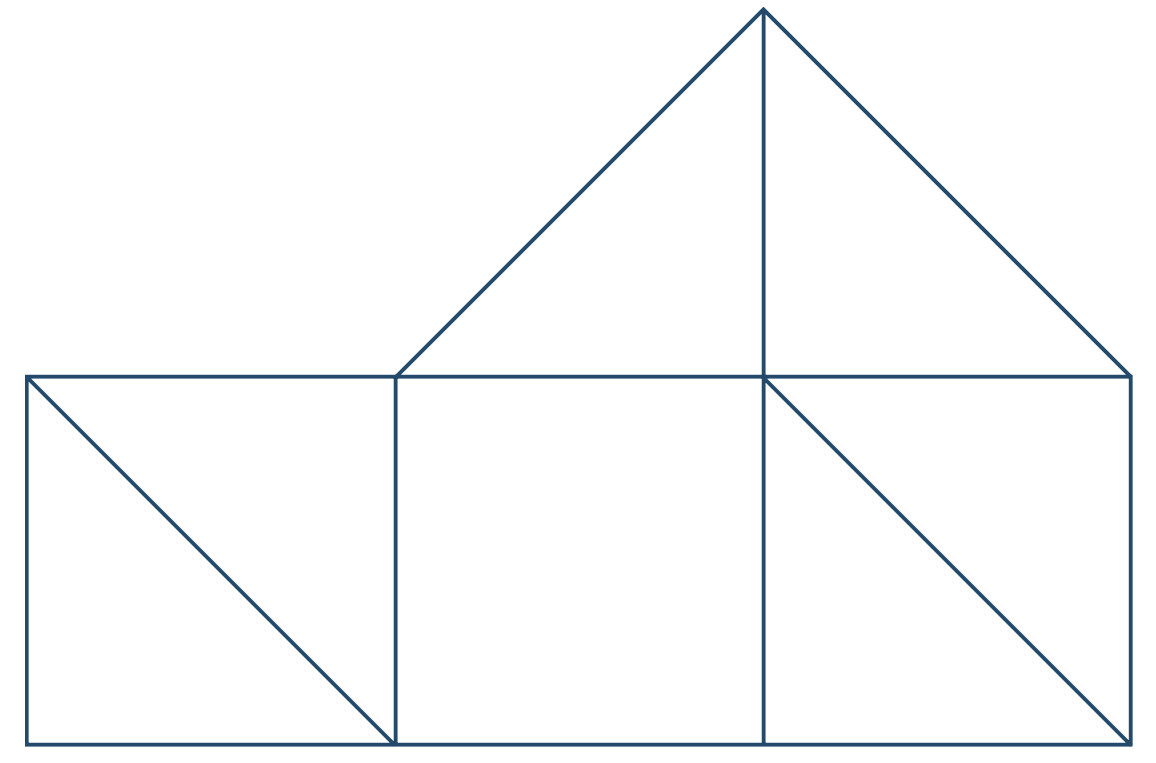
\includegraphics[width=0.5\textwidth]{figures/nodes.png}
\end{exercise}

\ifshowsolutions
\begin{solution}
There are $n = 9$ nodes, corresponding to the junctions.

There are $b = 15$ branches, corresponding to the individual segments connecting two nodes.

There are overall $l = 15$ geometric loops, i.e., closed paths. But only $m = b - n + 1 = 7$ of these closed paths are independent loops. One could choose the $7$ meshes (smallest possible loops, not enclosing any other loop) for an electrical network analysis, but other combinations are also possible.
\end{solution}
\fi

% ----- Exercise 3 -----
\begin{exercise}[Network Analysis 2]
The following network contains the resistors $R_1 = 1\,\Omega$, $R_2 = 2\,\Omega$, $R_3 = 5\,\Omega$, $R_4 = 25\,\Omega$, and $R_5 = 40\,\Omega$, as well as the source voltages $U_{q1} = 16.2\,\mathrm{V}$ and $U_{q2} = 11.4\,\mathrm{V}$. All branch currents are to be determined.

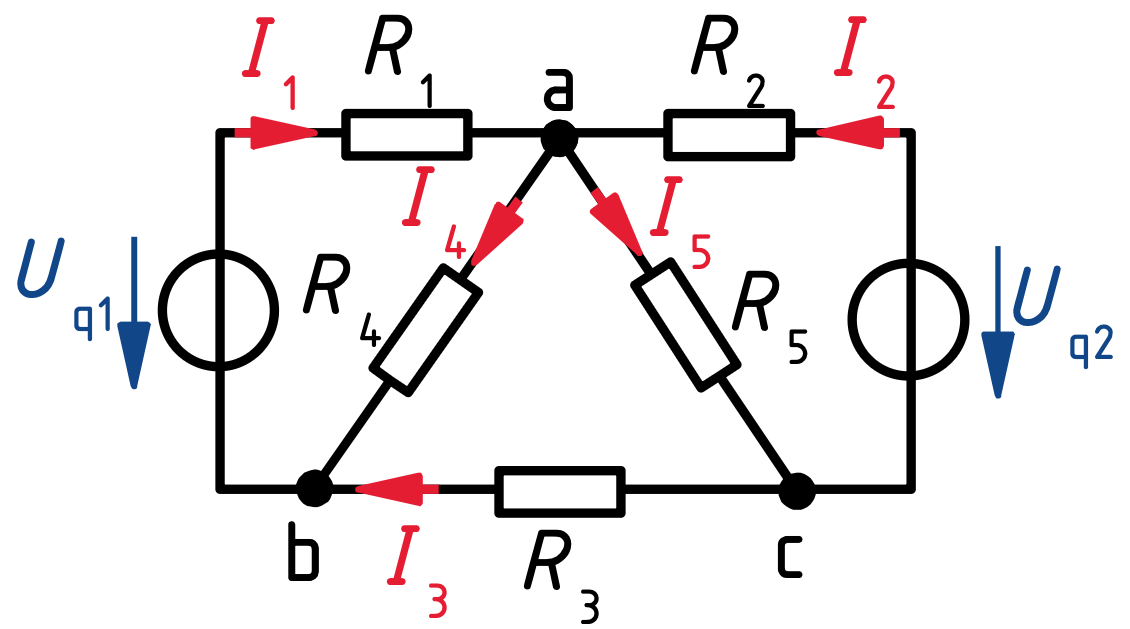
\includegraphics[width=0.7\textwidth]{figures/complete_tree_1.png}
\end{exercise}

\ifshowsolutions
\begin{solution}
This network has $n = 3$ nodes, so there are $n - 1 = 2$ linearly independent node equations. Picking nodes $B$ and $C$:
\[
I_3 + I_4 - I_1 = 0
\]
\[
I_5 - I_2 - I_3 = 0
\]

The number of branches is 5, so there are $5 - (3 - 1) = 3$ linearly independent mesh equations. Graph of the network with a selected complete tree (marked in red):

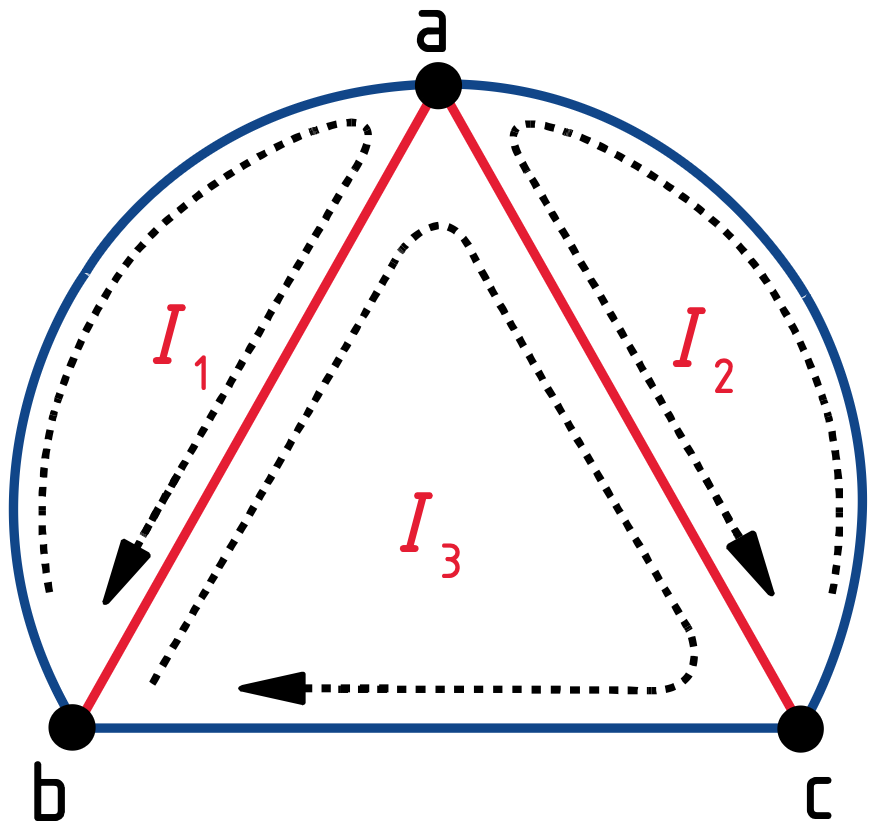
\includegraphics[width=0.4\textwidth]{figures/complete_tree_2.png}

The branch currents in the connecting branches, i.e., $I_1$, $I_2$, and $I_3$, are chosen as mesh currents. The mesh equations are set up by traversing the meshes in the direction of the counting arrows of the mesh currents:
\[
\begin{aligned}
M_1 &: \quad R_1 I_1 + R_4 I_4 - U_{q1} = 0 \\
M_2 &: \quad R_2 I_2 + R_5 I_5 - U_{q2} = 0 \\
M_3 &: \quad R_3 I_3 - R_4 I_4 + R_5 I_5 = 0
\end{aligned}
\]

Resulting system of equations as matrix equation:
\[
\begin{bmatrix}
-1 & 0 & 1 & 1 & 0 \\
0 & -1 & -1 & 0 & 1 \\
R_1 & 0 & 0 & R_4 & 0 \\
0 & R_2 & 0 & 0 & R_5 \\
0 & 0 & R_3 & -R_4 & R_5
\end{bmatrix}
\begin{bmatrix}
I_1 \\[4pt] I_2 \\[4pt] I_3 \\[4pt] I_4 \\[4pt] I_5
\end{bmatrix}
=
\begin{bmatrix}
0 \\[4pt] 0 \\[4pt] U_{q1} \\[4pt] U_{q2} \\[4pt] 0
\end{bmatrix}.
\]
Substituting numerical values gives:
\[
\begin{bmatrix}
-1 & 0 & 1 & 1 & 0 \\
0 & -1 & -1 & 0 & 1 \\
1 & 0 & 0 & 25 & 0 \\
0 & 2 & 0 & 0 & 40 \\
0 & 0 & 5 & -25 & 40
\end{bmatrix}
\begin{bmatrix}
I_1 \\[4pt] I_2 \\[4pt] I_3 \\[4pt] I_4 \\[4pt] I_5
\end{bmatrix}
=
\begin{bmatrix}
0 \\[4pt] 0 \\[4pt] 16.2 \\[4pt] 11.4 \\[4pt] 0
\end{bmatrix}.
\]
...
\[
I_1 = 1.2\,\mathrm{A}, \qquad
I_2 = -0.3\,\mathrm{A}, \qquad
I_3 = 0.6\,\mathrm{A}, \qquad
I_4 = 0.6\,\mathrm{A}, \qquad
I_5 = 0.3\,\mathrm{A}.
\]
\end{solution}
\fi

% ----- Exercise 4 -----
\begin{exercise}[Nodal Analysis]

Given the DC network with $U = 20\,\mathrm{V}$, $R_1 = 5\,\Omega$, $R_2 = 10\,\Omega$, $C = 100\,\mu\mathrm{F}$:

\begin{center}
\begin{circuitikz}[european, scale=1]
  \draw
  % Spannungsquelle
  (0,0) to[V, l_=$U$] (0,4)

  % R1
  (0,4) to[R=$R_1$] (4,4)

  % Knoten
  (4,4) node[circle,fill,inner sep=2pt] {}

  % R2
  (4,4) to[R=$R_2$] (8,4)
        -- (8,0)

  % Kondensator
  (4,4) to[C=$C$] (4,0)

  % Masse
  (0,0) -- (8,0);
\end{circuitikz}
\end{center}

The lower conductor is chosen as reference potential (ground). The steady-state condition ($t \rightarrow \infty$) is assumed.

Determine:

\begin{enumerate}
  \item the node voltage at the marked node,
  \item the voltage across the capacitor,
  \item the current through the capacitor,
  \item the energy stored in the capacitor.
\end{enumerate}
\end{exercise}

\ifshowsolutions
\begin{solution}
\[
\frac{V - U}{R_1} + \frac{V - 0}{R_2} = 0
\]
\[
2(V - 20) + V = 0
\]
\[
V = \frac{40}{3} \approx 13.33\,\text{V}
\]
\[
U_C = V - 0 = 13.33\,\text{V}
\]
\[
i_C = C \frac{du_C}{dt} = 0
\]
\[
W = \frac{1}{2} C U_C^2 \approx 8.9\,\text{mJ}
\]
\end{solution}
\fi

% ----- Exercise 5 -----
\begin{exercise}[Node Connection]
Calculate $I_o$ and $V_o$.

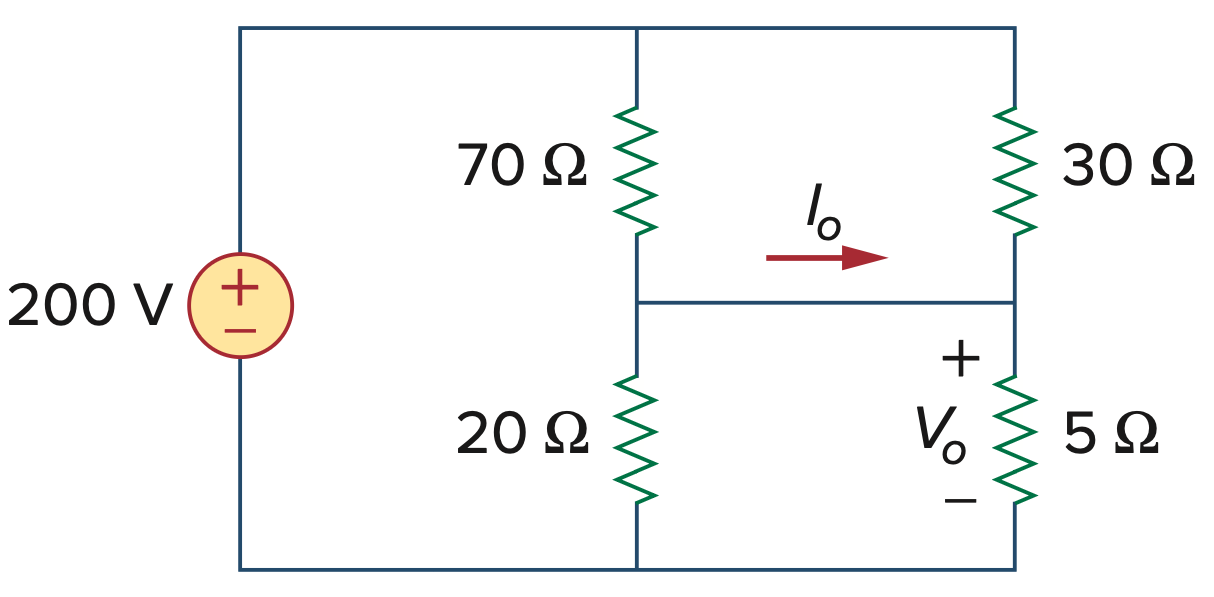
\includegraphics[width=0.7\textwidth]{figures/node_connection.png}
\end{exercise}

\ifshowsolutions
\begin{solution}
A node is a point where two or more circuit elements connect (electrically the same point). A branch is a path that connects two nodes and contains a circuit element (resistor, source, etc.).

Here, there are three main nodes:
\begin{itemize}
  \item Top node: connected to the $+200\, \mathrm{V}$ source, top of the $70\, \Omega$ and $30\, \Omega$ resistors.
  \item Bottom node: $0\, \mathrm{V}$ reference.
  \item Middle node: connection between two branches. On the left, the branch formed by the $70\, \Omega$ and $20\, \Omega$. And on the right, the branch formed by the $30\, \Omega$ and $5\, \Omega$.
\end{itemize}

The middle horizontal wire (with $I_o$) is part of the middle node, but because there’s a potential difference between the left and right parts of that node before it’s connected, current flows through that connection — hence we analyze $I_o$ as if it’s a branch current.

As the output voltage \(V_o\) is the voltage across the $5\, \Omega$ resistor, the output voltage equals the middle node voltage.

\[
\text{Currents from the top node to the middle node:}
\]
\[
I_{70} = \frac{200\, \mathrm{V} - V_o}{70\, \Omega}, \qquad I_{30} = \frac{200\, \mathrm{V} - V_o}{30\, \Omega}
\]

\[
\text{Currents from the middle node to the bottom node:}
\]
\[
I_{20} = \frac{V_o}{20\, \Omega}, \qquad I_{5} = \frac{V_o}{5\, \Omega}
\]

Applying KCL at the middle node:
\[
\frac{200\, \mathrm{V} - V_o}{70\, \Omega} + \frac{200\, \mathrm{V} - V_o}{30\, \Omega} = \frac{V_o}{20\, \Omega} + \frac{V_o}{5\, \Omega}
\]

Simplify:
\[
\frac{200\, \mathrm{V} - V_o}{21\, \Omega} = \frac{V_o}{4\, \Omega}
\]

\[
\Rightarrow 800\, \mathrm{V} - 4 \cdot V_o = 21 \cdot V_o
\]

\[
\Rightarrow \boxed{V_o = 32~\text{V}}
\]

Now we use KCL to compute the current \( I_o \) (defined to the right):

\[
I_o = I_{70} - I_{20} = \frac{200\, \mathrm{V} - 32\, \mathrm{V}}{70\, \Omega} - \frac{32\, \mathrm{V}}{20\, \Omega} =\boxed{0.8\, \mathrm{A}}
\]
\end{solution}
\fi

% ----- Exercise 6 -----
\begin{exercise}[Thévenin and Power Matching]
The variable resistor $R$ is adjusted until it absorbs the maximum power from the circuit.
\begin{enumerate}[label=\alph*)]
    \item Calculate the value of $R$ for maximum power.
    \item Determine the maximum power absorbed by $R$.
\end{enumerate}

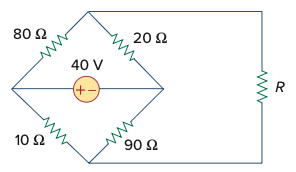
\includegraphics[width=0.7\textwidth]{figures/maximum_power.png}
\end{exercise}

\ifshowsolutions
\begin{solution}
\begin{enumerate}[label=\alph*)]
\item First, we calculate the Thévenin equivalent seen from the terminals of R.

Let node $D$ (left of $40\, \mathrm{V}$ source) be at $40\, \mathrm{V}$, and node $B$ (right of source) be at $0\, \mathrm{V}$.

For the upper node $A$:
\[
\frac{V_A - 40}{80} + \frac{V_A - 0}{20} = 0
\Rightarrow 5 V_A - 40 = 0
\Rightarrow V_A = 8\, \mathrm{V}
\]

For the lower node $C$:
\[
\frac{V_C - 40}{10} + \frac{V_C - 0}{90} = 0
\Rightarrow 10 V_C - 360 = 0
\Rightarrow V_C = 36\, \mathrm{V}
\]

Thus, the open-circuit (Thévenin) voltage is:
\[
V_\mathrm{th} = |V_A - V_C| = |8 - 36| = 28\, \mathrm{V}
\]

Now we deactivate the $40\, \mathrm{V}$ source (replace by a short circuit):
\[
R_A = (80\, \Omega \parallel 20\, \Omega) = \frac{80 \cdot 20}{80 + 20} = 16\, \Omega
\]
\[
R_C = (10\, \Omega \parallel 90\, \Omega) = \frac{10 \cdot 90}{10 + 90} = 9\, \Omega
\]

Since $R_A$ and $R_C$ are in series,
\[
R_\mathrm{th} = R_A + R_C = 16 + 9 = 25\, \Omega.
\]

For maximum power: $R = R_\mathrm{th} = 25\, \Omega$

\item The circuit can be represented by a Thévenin voltage source $V_\mathrm{th}$ in series with a Thévenin resistance $R_\mathrm{th}$ and a load $R_L$.
\[
I = \frac{V_{\text{th}}}{R_{\text{th}} + R_L}
\]

Power in the load:
\[
P = I^2 R_L = \frac{V_\mathrm{th}^2 R_L}{(R_\mathrm{th} + R_L)^2}
\]

Substitute $R_L = R_\mathrm{th}$ into the power equation:
\[
P_{\max} = \frac{V_\mathrm{th}^2 R_\mathrm{th}}{(R_\mathrm{th} + R_\mathrm{th})^2} = \frac{V_\mathrm{th}^2}{4 R_\mathrm{th}} = \frac{28^2}{4 \cdot 25} = \frac{784}{100} = 7.84\, \mathrm{W}
\]
\end{enumerate}
\end{solution}
\fi

% ----- Exercise 7 -----
\begin{exercise}[Efficiency]
Given the efficiencies listed below, determine the corresponding fraction of the maximum load power for each case.
\begin{enumerate}[label=\alph*)]
    \item $\eta = 75\%$
    \item $\eta = 90\%$
\end{enumerate}
\end{exercise}

\ifshowsolutions
\begin{solution}
Efficiency $\eta$ is defined as the ratio of power delivered to the load to the total power supplied by the source.

For a Thévenin source ($V_\mathrm{th}$, $R_\mathrm{th}$) with a load $R_L$, the efficiency is:
\[
\eta = \frac{P_L}{P_L + P_\mathrm{th}} = \frac{R_L}{R_L + R_\mathrm{th}}
\]

At maximum power ($R_L = R_\mathrm{th}$): 
\[
P_{L,\max} = \frac{V_\mathrm{th}^2}{4 R_\mathrm{th}}
\]

Hence, the power ratio is:
\[
\frac{P_L}{P_{L,\max}} = \frac{ \dfrac{V_\mathrm{th}^2 R_L}{(R_\mathrm{th} + R_L)^2} }{ \dfrac{V_\mathrm{th}^2}{4 R_\mathrm{th}} } = 4 R_\mathrm{th} \cdot \frac{R_L}{(R_\mathrm{th} + R_L)^2}
\]

\begin{enumerate}[label=\alph*)]
\item For $\eta = 75\%$:
\[
0.75 = \frac{R_L}{R_L + R_\mathrm{th}}
\]
\[
\Rightarrow R_L = 3 R_\mathrm{th}
\]
\[
\Rightarrow \frac{P_L}{P_{L,\max}} = 4R_\mathrm{th} \cdot \frac{3R_\mathrm{th}}{(R_\mathrm{th} + 3R_\mathrm{th})^2} = \frac{12R_\mathrm{th}^2}{(4R_\mathrm{th})^2} = 0.75
\]
Even when efficiency increases to 75\%, the load still receives 75\% of the maximum possible power. Thus, higher efficiency is achieved at the cost of only a moderate reduction in power delivered to the load.
\item For $\eta = 90\%$:
\[
0.9 = \frac{R_L}{R_L + R_\mathrm{th}}
\]
\[
\Rightarrow R_L = 9 R_\mathrm{th}
\]
\[
\Rightarrow \frac{P_L}{P_{L,\max}} = 4 R_\mathrm{th} \cdot \frac{9 R_\mathrm{th}}{(R_\mathrm{th} + 9 R_\mathrm{th})^2} = \frac{36 R_\mathrm{th}^2}{(10 R_\mathrm{th})^2} = 0.36
\]
So as efficiency rises, delivered power drops sharply.
\end{enumerate}
\end{solution}
\fi

% ----- Exercise 8 -----
\begin{exercise}[Power Measurement]
Calculate the effect of voltmeter and ammeter placement on the measured power in a DC resistive circuit with the parameters and configuratons below. Compare the measured power to the true power dissipated in the load resistor for both configurations and for the two different load resistances.

\begin{itemize}
  \item Source voltage: $V_s = 12\, \mathrm{V}$
  \item Source internal resistance: $R_s = 1\, \Omega$
  \item Voltmeter internal resistance: $R_v = 1000\, \Omega$
  \item Ammeter internal resistance: $R_a = 0.1\, \Omega$
  \item Load resistance (two cases):
  \begin{itemize}
      \item Low load resistance: $R_L =  1\, \Omega$
      \item High load resistance: $R_L = 100\, \Omega$
  \end{itemize}
\end{itemize}

\begin{enumerate}
  \item Configuration A (Current-corrected):\\
  Voltmeter connected across the source, ammeter in series with the load.\\

\begin{center}
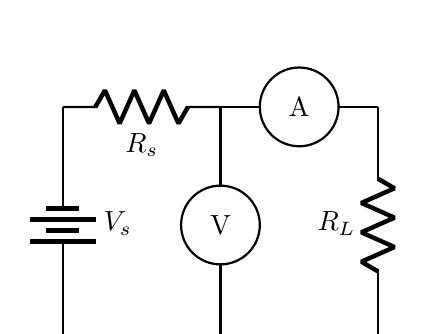
\begin{tikzpicture}[thick, scale=1.0]
  % Source with internal resistance
  \draw (0,0) to[battery, l_={$V_s$}] (0,3);
  \draw (0,3) to[resistor, l_={$R_s$}] (2,3);

  % Ammeter (as a circle)
  \draw (2,3) -- (2.5,3);
  \draw (3,3) node[circle,draw,minimum size=10mm,inner sep=0pt]{A};
  \draw (3.5,3) -- (4,3);

  % Load resistor
  \draw (4,3) to[resistor, l_={$R_L$}] (4,0);

  % Return path
  \draw (4,0) -- (0,0);

  % Voltmeter (as a circle)
  \draw (2,1.5) node[circle,draw,minimum size=10mm,inner sep=0pt]{V};
  \draw (2,0) -- (2,1);
  \draw (2,2) -- (2,3);
\end{tikzpicture}
\end{center}

  \item Configuration B (Voltage-corrected):\\
  Voltmeter connected across the load, ammeter in series with the source.\\
\end{enumerate}
\end{exercise}

\ifshowsolutions
\begin{solution}
\paragraph{Configuration A}
\[
I_s = I_L + I_v
\]
\[
I_L=\frac{V_t}{R_a + R_L}\quad\text{(through ammeter and load)}
\]
\[
I_v=\frac{V_t}{R_v}\quad\text{(through voltmeter)}.
\]

Source terminal relation:
\[
V_t = V_s - R_s \cdot I_s = \frac{V_s}{1 + R_s \left(\frac{1}{R_a + R_L} + \frac{1}{R_v}\right)}
\]

Measured power (what you would calculate from the meter readings, i.e.\ voltmeter~$\times$~ammeter):
\[
P_{\text{meas},A} = V_t I_L = \frac{V_t^2}{R_a + R_L} = \frac{V_s^2}{(R_a + R_L) (1 + R_s \left(\frac{1}{R_a + R_L} + \frac{1}{R_v}\right)^2}
\]

True power dissipated in load resistor:
\[
P_\text{true}=I_L^2 R_L = \dfrac{V_t^2\,R_L}{(R_a + R_L)^2}
\]

\paragraph{Configuration B}
\[
R_p = \frac{R_L R_v}{R_L + R_v} \quad\text{(parallel combination of load and voltmeter)}
\]
\[
I_s = \frac{V_s}{R_s + R_a + R_p}
\]
\[
V_L = I_s \, R_p \quad\text{(voltage across load and voltmeter)}
\]

Measured power:
\[
P_{\text{meas},B} = V_L I_s = I_s^2 R_p = \frac{V_s^2 R_p}{(R_s + R_a + R_p)^2}
\]

True power dissipated in load resistor:
\[
P_\text{true} = I_L^2 R_L
\]
\[
I_L = \frac{V_L}{R_L} = \frac{I_s R_p}{R_L}
\]
\[
\Rightarrow P_\text{true} = \frac{I_s^2 R_p^2}{R_L}
\]

\begin{center}
\begin{tabular}{lrrrrr}
\hline
$R_L$ & $P_\text{true}$ & $P_{\text{meas},A}$ & $P_{\text{meas},B}$ \\
\hline
$1\, \Omega$ & $32.62\, \mathrm{W}$ & $35.88\, \mathrm{W}$ & $32.65\, \mathrm{W}$ \\
$100\, \Omega$ & $1.406\, \mathrm{W}$ & $1.407\, \mathrm{W}$ & $1.546\, \mathrm{W}$ \\
\hline
\end{tabular}
\end{center}
\end{solution}
\fi

\end{document}